%!TEX root = main.tex
\chapter{Expérimentations}
\chaptertable

\section{Cas d'étude : Assemblage collaboratif d'objets 3D dans un 
environnement web}

Dans le cadre de la modélisation 3D collaborative, il existe plusieurs types 
d'application comme nous l'avons vu (\gls{CAO} collaborative, \gls{BIM} \dots). 
Ces domaines d'activité ont un point en commun, les fonctionnalités de 
modélisation 3D qui sont récurrentes sont les cas d'assemblage d'objets 3D de 
manières collaborative. Dans la mise en situation, les utilisateurs ont déjà une 
modélisation précise de leur modèle sur leur machine qu'ils ont par exemple 
réalisé à l'aide de logiciels spécifiques. L'utilisateur est responsable de fournir un 
modèle compatible avec le prototype notamment concernant le format et la taille 
du fichier et la sécurité du modèle qu'il partage (tatouage, droits). Le cas d'étude 
présente la mise en commun de ces objets pré-conçus dans un environnement 
web.

L'\textbf{expérimentation 1} concerne l'expérimentation réalisée dans 
\cite{Desprat2015a} 
et \cite{Desprat2015b}. Elle utilise le prototype décrit dans la Section \todo{ref 
section} et s'intéresse à montrer une preuve de faisabilité concernant l'architecture 
de communication décrite dans la section \ref{sec:comm_state}. 

 
L'\textbf{expérimentation 2} concerne l'expérimentation réalisée dans 
\cite{Desprat2016} et 
\cite{Desprat2017}. Elle utilise le prototype décrit dans la Section \todo{ref section} 
et s'intéresse à montrer l'intérêt auprès des utilisateurs d'une \gls{EDA} pour la 
visualisation et la manipulation d'objets 3D reposant sur le modèle 
événementiel présenté dans la section \ref{sec:modele_event} et les 
répercussions sur l'architecture de 
communication décrite dans la section \ref{sec:comm_event}.


Globalement, les objectifs des expérimentations menées au cours de la thèse 
soulignent 
plusieurs aspects relatif à la fiabilité 
du modèle et de 
son implantation de deux manières: 
\begin{itemize}
	\item fonctionnelle : manipulation et visualisation 
	3D, historique ;
	\item et technique : récupération de l'information, cohérence des 
	données, disponibilité du réseau.
\end{itemize}

\section{Expérimentation 1 : preuve de faisabilité}

Ce cas d'étude présenté dans \cite{Desprat2015a, Desprat2015b} présente 
une preuve de concept concernant l'architecture de communication : qu'est-ce 
qu'apporte une architecture hybride dans la collaboration temps réel ? Est-il 
possible techniquement de réaliser une 
telle architecture pour l'échange de ressources 3D de manière fiable et efficace 
uniquement avec des technologies web? Quels sont les apports pour la 
collaboration, les utilisateurs et la réalisation de la tâche?
Un des objectifs de cette expérimentation est de démontrer la faisabilité de notre 
approche réseau hybride avec une attention particulière à l'égard de l'expérience 
utilisateur.


%!TEX root = main.tex
%\section{Assemblage d'objets 3D sur le web avec architecture 
%événementielle}
%\label{sec:us}

\subsection{Présentation de l'expérimentation}

L'expérimentation propose de répliquer une collaboration réaliste entre 
différents participants travaillant à distance pour faire des tâches d'assemblage de 
modèle 3D. L'expérimentation reprend le cas d'étude de l'assemblage d'objets 3D 
(Section \ref{xp:use_case}). 

L'expérimentation est basée sur un prototype d'application développé selon 
l'implantation présentée dans la Section \todo{ref section proto}.
Le prototype est développé sur une plateforme web et consiste en un application 
de modélisation 3D collaborative multi-utilisateurs pour démontrer la faisabilité de 
l'architecture présentée dans \todo{ref section archi state}. 


\paragraph{Tâches à effectuer.}
L'expérimentation consiste en quatre épreuves qui partagent la même procédure.
Les modèles utilisés dans chaque épreuve sont décrits dans le tableau 
\ref{table:models_xp1} : \textit{Wind Turbine}, \textit{Pick up} et \textit{Castle}. 

Les épreuves sur les modèles \textit{Wind Turbine} et \textit{Pick Up} partagent le 
même objectif : 
assembler un modèle, dont les utilisateurs possède l'image, composé de 
différentes pièces qui sont téléversées par les utilisateurs. L'image correspond à 
l'assemblage final à obtenir et indique les différentes parties qui le 
compose (type et quantité). Ces deux épreuves s'arrêtent lorsque les participants 
le notifient oralement ou durent dix minutes maximum chacune.

Le modèle \textit{Castle} est utilisé dans deux épreuves : 
\textit{Castle from server} et \textit{Castle from peer}. L'objectif de ces épreuves
diffère un peu des épreuves précédentes car l'épreuve s'effectue sur un  modèle 
de château en kit (composer d'un dizaine d'objets différents : tour, murs, 
escalier\dots) : les 
participants ont dix minutes pour construire un 
château de manière collaborative en faisant appel à leur créativité. 
Dans l'épreuve \textit{Castle from server}, les objets sont récupérés 
automatiquement à partir du serveur ; 
dans l'épreuve \textit{Castle from peer}, les pairs peuvent ajouter de nouveaux 
objets du kit qu'ils possèdent sur leur machine.

En utilisant les outils de l'éditeur, les informations liées aux autres utilisateurs 
(représentation dans l'environnement 3D de leur position ou de leur sélection), les 
utilisateurs doivent manipuler les pièces (sélection, rotation, translation, 
homothétie) de manière collaborative afin d'atteindre l'objectif. 
\paragraph{Population}
L'expérience a été conduite sur trois groupes de trois ou quatre participants 
chacun. Un essai pour \textit{Wind Turbine} a été tenté à six participants 
simultanés.
Durant l'expérimentation, les utilisateurs était sur le même réseau que le serveur 
(\gls{LAN}). 
Les participants étaient des étudiants de Master ou de Doctorat en Informatique 
plutôt familiers avec les environnements 3D. Les participants étaient autorisés à 
communiquer entre eux (oralement, par chat, autre \dots).
\paragraph{Procédure}
L'expérimentation consiste en quatre épreuves qui partagent la même procédure:
\begin{enumerate}
	\item Phase d'essai 
	\begin{enumerate}
		\item explication du contexte et de l'expérimentation ;
		\item prise en main du système, familiarisation avec 
		l'interface ;
	\end{enumerate}
	\item Phase de collaboration : réalisation de l'épreuve (se répète autant de fois 
	que d'épreuves)
	\begin{enumerate}
		\item Présentation de l'épreuve et de son objectif
		\item Initialisation : nettoyage de la scène et chargement des modèles
		\item Réalisation de l'objectif
	\end{enumerate}
	\item Phase de retour d'expérience : remplissage questionnaire et discussion 
	informelle sur les épreuves.
\end{enumerate}

\paragraph{Initialisation}

L'épreuve est décrite et l'objectif de l'épreuve est présenté a tous les participants.
Pour chaque phase de collaboration, l'application nettoie les données issues de 
l'épreuve précédente. 
À l'exception des pièces du modèle \textit{Castle} qui sont chargées
en totalité sur le serveur dans \textit{Castle from server} et les pairs \textit{Castle 
from peer}), les pièces du modèle de l'épreuve sont distribuées de manière 
aléatoire entre les différents participants.

\paragraph{Données collectées}
Au cours des épreuves (principalement lorsque celles ci s'arrêtent)  les 
participants ont exprimé certains retours qualitatifs dont il a été pris note. Le type 
d'interaction entre les participants est également observé.

\paragraph{Questionnaire}
Au début de l'expérimentation, les participants reçoivent et prennent connaissance 
du questionnaire (voir Annexe \ref{q:xp1}). Ce questionnaire est rempli à plusieurs 
moment au cours de l'expérimentation. Au début, le participant décrit sa situation, 
sa familiarité avec les environnements 3D, le type de machine et de navigateur 
qu'il utilise. À la fin de chaque épreuve il répond aux questions concernant 
l'épreuve qu'il vient de passer. À la fin de l'expérimentation, il répond aux 
questions d'ordre plus général sur son expérience et les améliorations 
envisageables.
\subsection{Résultats et discussion}
Les participants ont globalement été satisfaits des résultats issus de la 
collaboration ainsi que du rendu visuel des assemblages effectués durant les 
épreuves. Cela est également dû au fait qu'ils ont systématiquement atteint les 
objectifs (dans le temps imparti) : réalisation de l'assemblage du modèle 3D 
présenté sans frustration. Ils se sont également \og amusés\fg{} sur les épreuves
avec le \textit{Castle} car ils étaient libres dans la création et souhaiter continuer 
l'épreuve au delà du temps imparti. L'utilisation de canaux de communication 
externes à l'application a été reportée plusieurs fois, principalement sous formes 
d'échanges oraux. Ces échanges concernait l'état de leur application et ce qu'ils 
étaient en train de faire ou ce qu'ils souhaitaient faire. Cette interaction provient, 
d'après les participants, du manque de retours visuels différenciés sur les 
manipulations effectués par les collaborateurs (exemple: pas de couleur différente 
pour sélection d'objet par un autre utilisateur). Cela peut plus généralement 
s'expliquer comme un manque sensibilisation à l'environnement collaboratif. 
L'\gls{IU} a été bien appréciée, parfois jugée \og trop simple\fg{} par certains 
utilisateurs. Ce choix avait été fait pour faciliter l'usage, l'apprentissage et 
l'adoption de l'\gls{IU} et s'est révélé anecdotique lors de l'expérimentation car le 
panel de personne de participants était familier de ce genre 
d'environnement (échantillon faible).
Les fonctionnalités liées à la manipulation d'objets reçoivent une bonne évaluation 
à l'exception de l'importation de modèles. Cela est dû, dans ce prototype, au 
fait que l'application ne peut digérer et transmettre des modèles trop lourds. Un 
participant a vu sa fenêtre \og geler\fg{} (navigateur Chrome) lors de l'épreuve 
\textit{Castle from peer}. Cela l'a amené à quitter la session et à revenir sur la 
scène pour pouvoir continuer de participer à la session collaborative. Sans 
perturber la session en cours pour ses collaborateur, le participant a pu revenir sur 
l'application, reprenant la collaboration avec les autres participants (rétablissement 
des connexions après un crash).En cela le participant a apprécié la robustesse de 
l'application sans être perturbé très longtemps par l'interruption.
Concernant la fluidité des manipulations et de la visualisation au sein de 
l'application durant la collaboration, les participants n'ont pas ressenti de latence 
perturbantes en général. Ils ont qualifié l'application de temps-réel plutôt 
qu'interactive. La variation du nombre d'utilisateur sur les différentes épreuves n'a 
pas altéré la qualité du rendu et de réseau pour le participant.

\subsection{Conclusion de l'expérimentation 1}

This paper proposed web-based 3D modeling collab- oration based on a hybrid 
communication architecture client-server and P2P network. The client is respon- 
sible for 3D rendering and handling the user interac- tions on a scene. It also hosts 
the peer connection to be able to communicate updates to other peers. The server 
is used to link the client with the NoSQL database in order to store the 
modifications, and manage the users presence on a scene and automatically 
create a P2P full mesh topology network between them. The P2P con- nection 
relies on a WebRTC communication that trans- mits information directly between 
browser with update messages, broadcasting according to the P2P star topol- ogy, 
using a signaling server to establish the commu- nication between two peers. The 
qualitative evalua- tions of the experiments were conclusive overall even if some 
points should be improved. On model import, the broadcast causes latency issues 
on client peers re- ceivers (camera freeze). To reduce latency with larger scenes 
we consider using progressive rendering and making a better use of peer-to-peer 
mesh to stream the model relying on seed peers like in the partial mesh topology. 
An improvement of interface features and visual feedback of collaborative 
manipulations was asked by the users. This evaluation will be supple- mented in 
future works with a quantitative evaluation to compare our hybrid architecture to 
others, particu- larly using server logs, FPS in client and WebRTC tools (Chrome : 
chrome://webrt-internal; Firefox : about:webrtc) which provides statistics and 
graphs on the data exchanged between peers’ browsers.
\section{Expérimentation 2 : Intégration du framework événementiel}
\label{sec:us}
%!TEX root = main.tex
%\section{Assemblage d'objets 3D sur le web avec architecture 
%événementielle}
%\label{sec:us}
L'expérimentation propose de répliquer une collaboration réaliste entre différents 
participants travaillant à distance. Ce cas d'étude présenté dans 
\cite{Desprat2017} souligne plusieurs aspects relatif à la fiabilité du modèle et de 
son implantation de deux manières: 
\begin{itemize}
	\item fonctionnelle : manipulation et visualisation 
	3D, historique ;
	\item et technique : récupération de l'information, cohérence des 
	données, disponibilité du réseau.
\end{itemize}

Quant à l'observation du comportement des participants, elle est 
effectuée de manière quantitative (outils de surveillance) et de manière qualitative 
(questionnaire) lors de l'exécution d'une tâche coopérative au sein de l'application.

%The 3D data issued from X (cite) represent the different parts of a 3D printed 
%case for a camera based on RaspberryPi and a Thermal Printer. Data used in 
%the 
%experiment are triangulated surfaces converted from the STL files given. The 
%case 
%is composed of N connected components. (see figure F).
\paragraph{Tâche à effectuer}
Les participants devaient assembler les différentes parties d'un modèle 3D en 
utilisant l'application 3DEvent et les fonctionnalités décrites précédemment 
\info{ref section foncitonnalités} pour que le résultat corresponde à l'assemblage 
donné en exemple (images). La complexité de la tâche a été modulée selon 
plusieurs facteurs : le nombre de parties composant le modèle et le nombre de 
collaborateurs. Afin de permettre la manipulation des objets 3D facile à 
apprendre et utiliser, il a été choisi de conserver des manipulations de haut niveau.
%Participants had to assemble in a web-browser the different parts of a model 
%using 3DEvent application and features described in Section \ref{sec:ui} to 
%match 
%a final given assembly. The complexity of the task was modulated by the 
%number 
%of parts composing the assembly and the number of collaborators. We wanted to 
%keep the 3D manipulation tasks at high level to be easy to learn/use.
\paragraph{Population}
L'expérience a été conduite sur 12 groupes de deux ou trois participants chacun. 
Chaque participant était localisé en France dans une zone urbaine avec de bonnes 
infrastructures en travaillant sur des réseaux distincts avec une bonne connexion 
internet (au moins 20Mb/s) pour éviter d'avoir des latences extrêmes (>10 
secondes) au cours 
des expérimentations. Les participants étaient des étudiants de Master ou de 
Doctorat en informatique (pas nécessairement familiers avec les environnements 
3D). Les participants étaient autorisés à communiquer entre eux par chat.


\paragraph{Procédure}
Les modèles utilisés lors de l'expériences sont décrits dans le Tableau 
\ref{table:summary}. L'expérimentation se déroule en trois phases : 
\begin{description}
	\item[Phase d'essai] Chaque participant s'entraîne pendant 5-10 minutes sur un 
	modèle de test dans l'application pour se familiariser avec l'interface et les 
	fonctionnalités proposées.
	\item[Phase solo] Le participant effectue un assemblage du modèle Rotor ou 
	Camera Box.
	\item[Phase de collaboration] Un groupe de participants réalise deux 
	assemblages sur 
	\begin{enumerate*}[label=(\roman*)]
		\item un petit modèle (10 ou 12 parties) puis
		\item un plus gros modèle (16 parties).
	\end{enumerate*}
	La phase de collaboration a été répétée six fois : trois fois 
	avec un groupe de deux participants et trois fois avec un groupe de trois 
	participants.
\end{description}

Du fait que les participants pouvaient participer à différentes configurations de 
groupe durant la phase de collaboration, plusieurs modèles 3D avec des 
caractéristiques similaires (nombre de parties et nombre de triangles) ont été 
présentés pour éviter les biais liés à l'apprentissage.

\begin{table}[ht]
	\centering
	\caption{Modèles utilisés durant l'expérimentation}
	\label{table:summary}
	\begin{tabular}{cccc}\hline
		\textbf{Modèle}  & \textbf{Nombre de parties} &  \textbf{Nombre de triangles} 
		& \textbf{Taille totale}  \\ \hline
		Rotor      &   10  &    62k & 4Mo        \\
		Camera box        &   12  &    67k & 5Mo        \\
		Car      &   16  &      170k & 8Mo \\       
		Living room      &   16  &      200k & 9Mo \\    \bottomrule
	\end{tabular}
\end{table}
\paragraph{Initialisation}

Pour chaque phase, l'application a été initialisée par le chargement des parties du 
modèle dans la bibliothèque d'objets chez chaque participant. Les parties des 
objets ont volontairement été positionnées (rotation et homothétie) aléatoirement 
afin que les utilisateurs aient à manipuler les différentes fonctionnalités. Cette 
configuration nous permet d'observer l'activité à l'intérieur de chaque groupe durant 
l'expérimentation. Chaque participant a reçu une image de l'assemblage à réaliser 
(la tâche à compléter). 

\paragraph{Données collectées}
Pour chaque expérimentation et chaque participant, le temps de complètement, le 
nombre d'événements générés et l'horodatage de chaque événement pour 
observer le complètement de la tâche en termes de vitesse et d'efficacité ainsi 
que les effets sur le temps d'implication d'un collaborateur selon le nombre de 
collaborateurs. 

L'enregistrement des données commence lorsque le premier événement sur la 
scène initialisée est généré (horodatage du premier événement); et il s'arrête 
lorsque le groupe indique que la tâche à compléter est terminée (horodatage du 
dernier événement est considéré).


\paragraph{Questionnaire}
En dehors des données collectées, les participants devaient remplir un 
questionnaire basé sur l'expérimentation pour exprimer leurs retours qualitatifs 
concernant leur expérience (Annexe \ref{app:quest}) \info{ajout questionnaire}. 

Le questionnaire est inspiré de \cite{Lewis1995}, qui permet d'évaluer la facilité 
d'utilisation du système et l'implication dans la collaboration de chacun des 
participants. En utilisant une échelle de notation sur sept points \cite{Lewis1993}, 
(1~:~pas d'accord~; 7~:~d'accord) pour avoir assez de points de discrimination.



Au cours des différentes sessions collaboratives, l'application à produit plusieurs 
centaines d'événements (environ 300 par session). Les expérimentations ont été 
réalisées sur plusieurs dispositifs notamment un \textit{smartphone} avec une 
connexion 4G. 
La Figure \ref{fig:screenshots} montre quelques captures d'écran durant une 
session collaborative sur le modèle Rotor ; et la Figure \ref{fig:ui4} montre les 
premiers événements enregistrés dans la base de données\info{mettre ailleurs?}. 
Les boîtes englobantes représentent la sélection des différents collaborateurs 
pendant la session.
\begin{figure}[ht]
	\centering
	
	\subfloat[Translation (environnement 3D) et visualisation de l'historique 
	(panneau 
	latéral)]{\includegraphics[width=0.7\textwidth]{eps/1translatehisto.eps}\label{fig:ui1}}\hfill
	\subfloat[Rotation (environnement 3D) et outils pour la manipulation d'objet 3D 
	(panneau 
	latéral)]{\includegraphics[width=0.7\textwidth]{eps/2rotatedetail.eps}\label{fig:ui2}}\hfill
	\subfloat[Mise à l'échelle (environnement 3D) et liste des collaborateurs 
	(panneau 
	latéral)]{\includegraphics[width=0.7\textwidth]{eps/3scalecollab.eps}\label{fig:ui3}}\hfill
	\caption{Interface utilisateur pendant une session collaborative (trois personnes)}
	\label{fig:screenshots}
\end{figure}

\begin{figure}[ht]
	\centering
	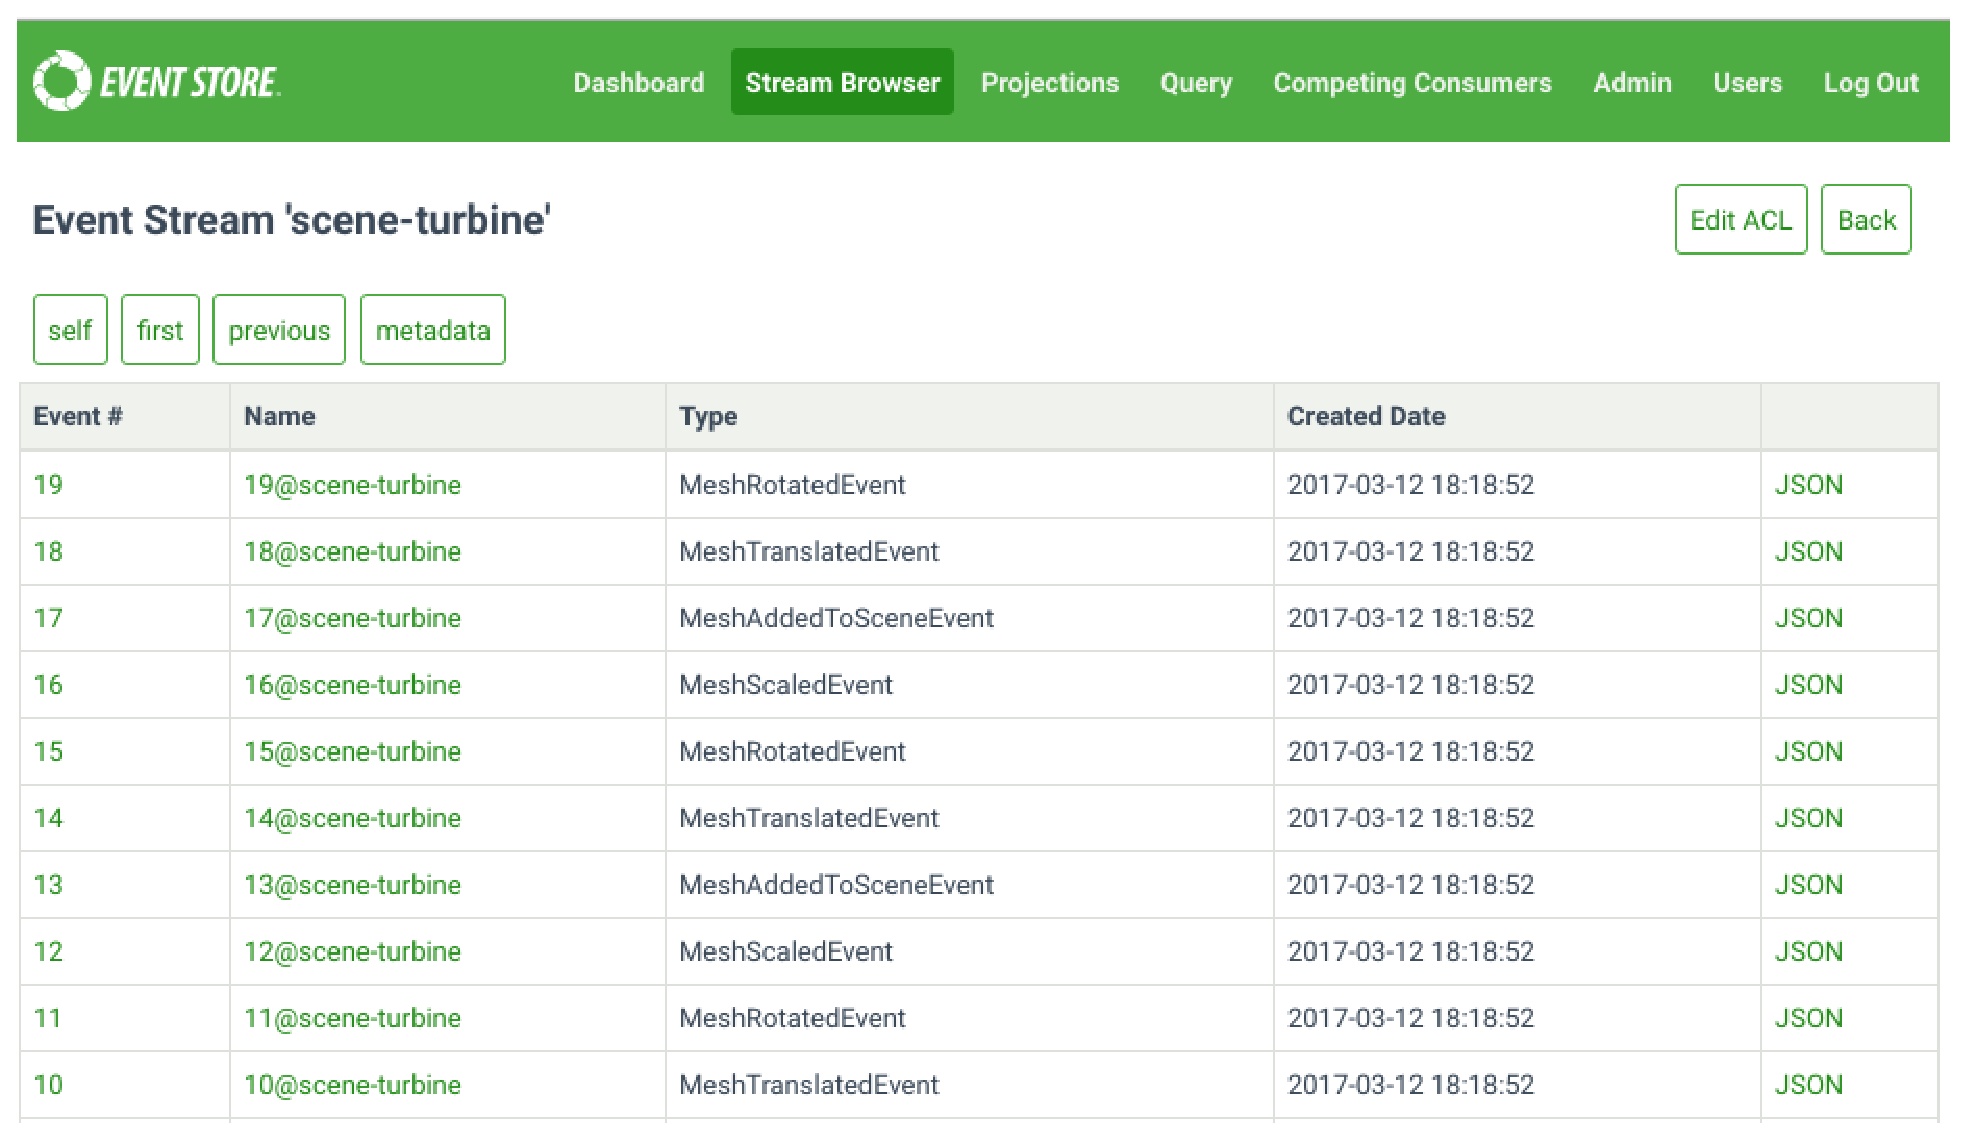
\includegraphics[width=\textwidth]{eps/eventstore.eps}
	\caption{Persistance long-terme (Event Store\textsuperscript{\textregistered}), 
		base de données/outil de monitoring}
	\label{fig:ui4}
\end{figure}

\subsection{Résultats et Discussion}
\label{sec:res}


\paragraph{Analyse des interactions}
Les traces des utilisateurs récupérées au cours des expérimentations sont la base 
du travail d'analyse qui est présenté ici. Ces traces, composées d'événements 
générés par les utilisateurs, permettent de savoir qui (Figure \ref{petita}) a fait quoi 
(Figure \ref{petitb}) lors des sessions collaborative. Généralement, le \og qui\fg{} 
est assez facile à retrouver lors de la récupération des traces. Le \og quoi\fg{} 
cependant nécessite que les notifications aient une signification précise et proche 
du métier. Grâce au travail de découpage et de dénomination des événements 
effectué en amont, le journal d'événements (\textit{log}) indique précisément tout 
ce 
qui s'est passé lors de la session du point de vue du métier. Cette fonctionnalité est 
intéressante dans le contexte de la traçabilité des données et lors d'audits sur 
l'assemblage. 

Figure \ref{fig:collabsession} montre deux angles d'enregistrement d'une session 
sur le modèle \textit{living room}. Au début de la session, beaucoup d'objets sont 
ajoutés (meshAddedToSceneEvent). Seul un utilisateur a ajouté un objet en 
utilisant la fonctionnalité pour déposer un objet à un endroit spécifique de la scène 
(meshDropped \info{name it}). Le nombre d'événements concernant la sélection et 
la désélection est à peu près similaire aux exception. La différence s'explique par 
le fait que l'événement de désélection n'est pas déclenché lors d'un changement 
d'objet sélectionné, car la désélection n'est pas effectuée explicitement par 
l'utilisateur. Au commencement, les participants ont fortement interagit (jusqu'à 20 
événements en 15 secondes). Cela s'explique par le recours massif à l'ajout 
d'objets dans la scène pour composer le modèle et la mise à l'échelle de ceux-ci 
(du au positionnement arbitraire des objets de la bibliothèque). Ensuite, les trois 
utilisateurs interagissent ensemble durant quelques minutes avant que l'un d'entre 
eux ne quitte et ne reviennent quelques secondes plus tard (informations 
récupérées à partir du journal d'événements lié aux agrégats utilisateurs). Enfin, le 
nombre d'événements diminue montrant la fin de l'activité, les utilisateurs finissant 
la tâche et ajustant les derniers objets.

L'implication d'un utilisateur peut être vue par le prisme de la fréquence de ses 
contributions et la variété de fonctionnalités utilisées, autrement dit, les différents 
types d'événement produits. L'analyse d'une session apporte plusieurs indicateurs 
tout au long de la session. Par exemple, l'absence d'un utilisateur pendant une 
longue période peut indiquer une déconnexion. Ou encore, l'utilisation trop 
fréquente d'un type d'événement (ou d'un motif d'événements répété) peut montrer 
une faiblesse de l'ergonomie de l'interface. Pour ce dernier aspect, on peut prendre 
l'exemple dans la Figure \ref{petitb} à 45s, on remarque un nombre élevé de 
MeshScaledEvent. A posteriori, nous nous sommes rendu compte que la 
fonctionnalité était mal calibrée pour l'échelle du modèle et nécessitait donc de s'y 
reprendre à de nombreuse fois pour réaliser la bonne transformation.

\begin{figure}[ht]
	\centering
	
	\subfloat[Par 
	utilisateur]{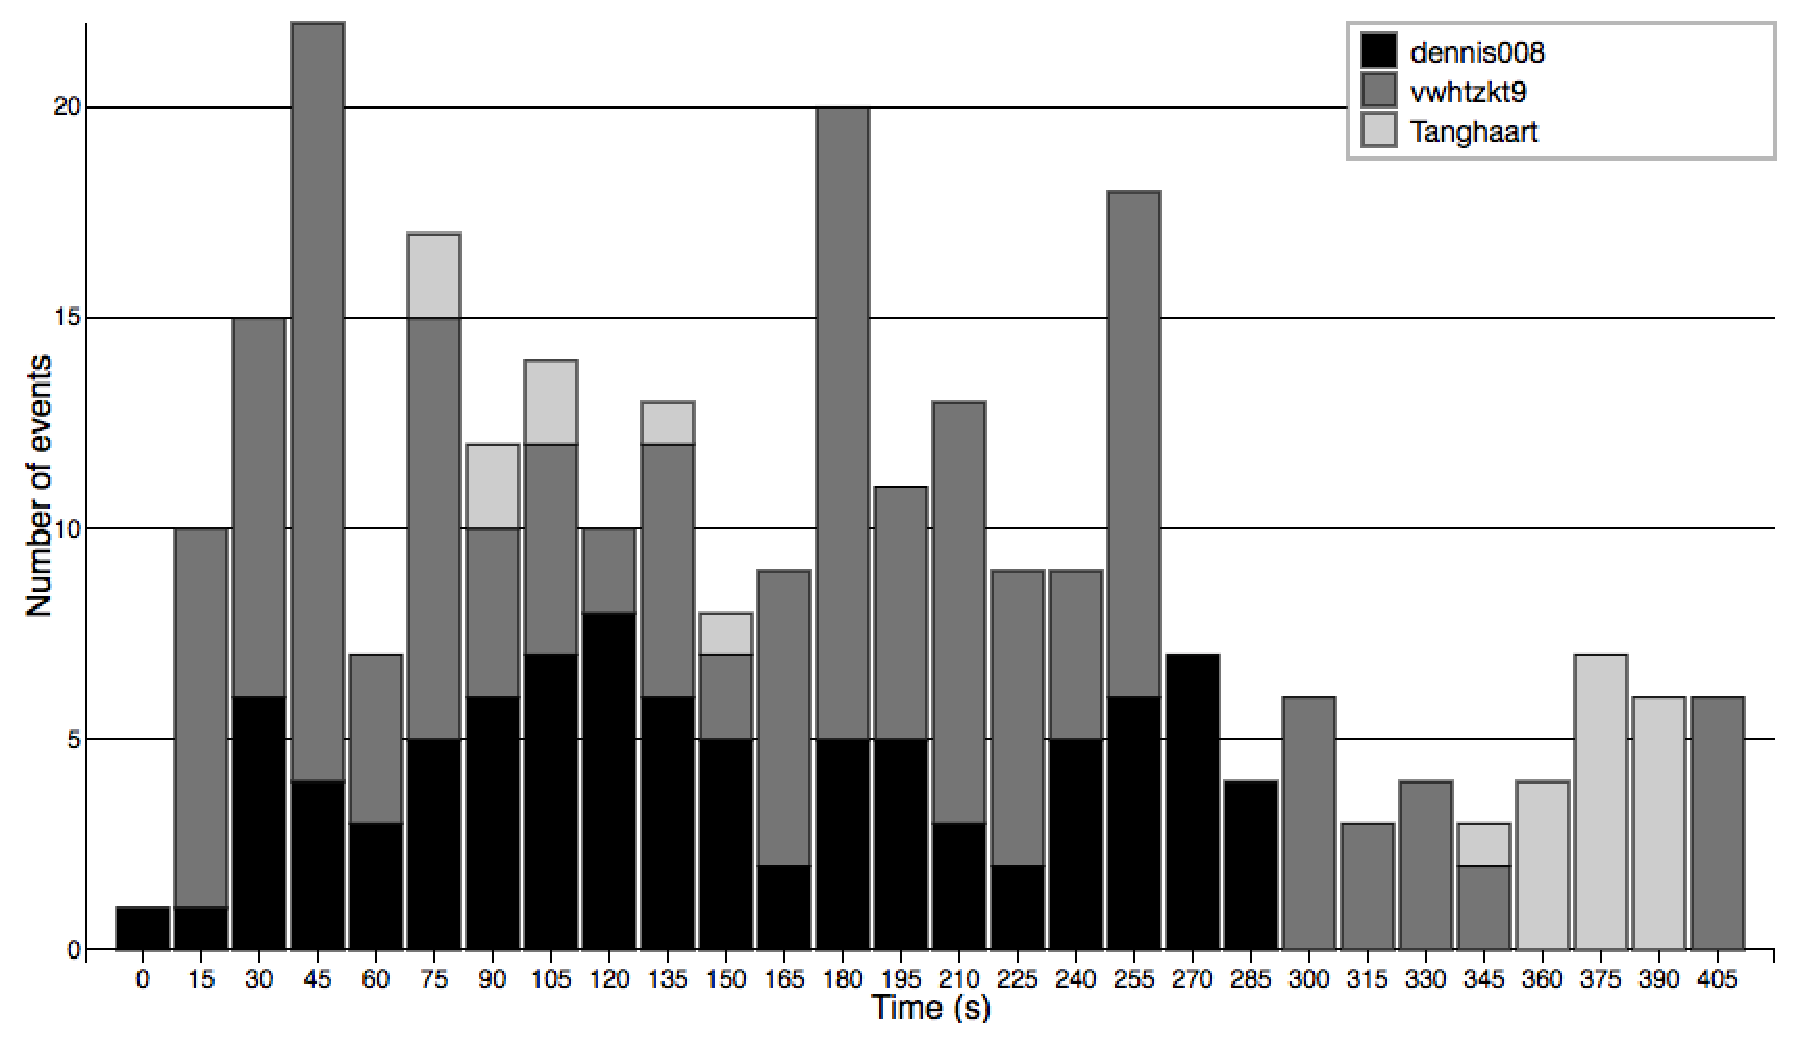
\includegraphics[width=\columnwidth]{eps/byuser.eps}\label{petita}} \\
	\subfloat[Par type 
	d'événement]{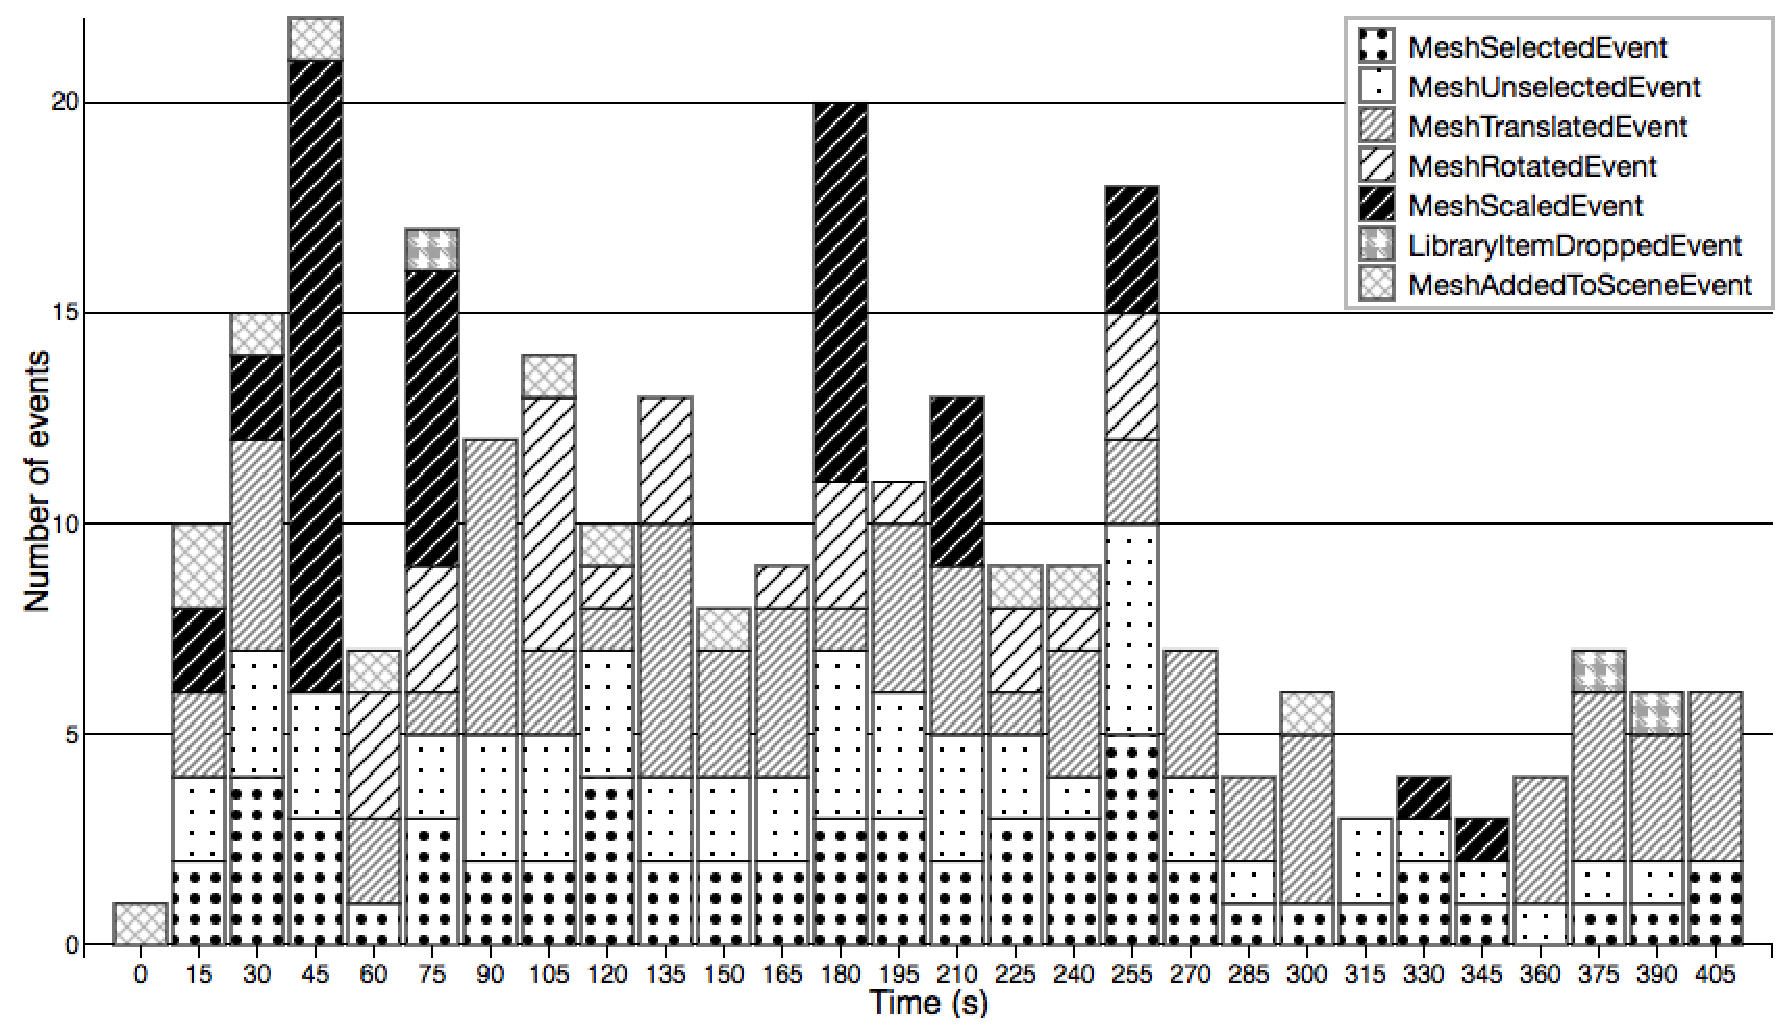
\includegraphics[width=\columnwidth]{eps/byevents.eps}\label{petitb}}
	\caption{Résumé d'une session collaborative au cours du temps}
	\label{fig:collabsession}
\end{figure}

\paragraph{Questionnaires}
Après chaque expérimentation, le participant a rempli directement un questionnaire 
à propos des phases solo et collaboratives qu'il a effectuées via le formulaire en 
ligne. les résultats obtenus sont compilés dans la Figure 
\ref{fig:questionnaire} sous la forme de boîte à moustache. Cette représentation 
est un moyen rapide de figurer le profil essentiel des résultats des mesures 
quantitatives effectuées.
Globalement, les tâches ont été réalisées plus rapidement et plus efficacement 
de manière collaborative que de manière solo. La facilité d'utilisation et la 
simplicité de l'interface sont également soulignées positivement par plusieurs 
utilisateurs. Comme indiqué dans les retours d'expérience négatifs, la stabilité du 
réseau a parfois amené un peu de frustration chez certains participants. 
Cependant, les participants ont trouvé que la cohérence de l'environnement lors de 
la collaboration et la récupération des données était plus qu'acceptable. Cette 
remarque s'accompagne également du fait que la distribution des données s'est 
effectuée correctement\info{proove it}, leur permettant de coopérer efficacement.

Durant l'une des expérimentations en phase collaborative, nous avons eu un 
participant avec une latence de plus de 10s à certains moment, mais malgré cela, 
le groupe nous a notifié que cela n'avait pas affecté la collaboration. Au long des 
expérimentations, quelques conflits ont été levés sur différentes opérations à 
différent niveaux. Au niveau réseau (mauvaise version, désynchronisation), la 
politique en place est d'annuler l'événement et de resynchroniser les utilisateurs 
entre eux. Au niveau des utilisateurs (opérations opposées sur le même objet), la 
résolution du conflit doit passer par un canal externe (chat) pour que les 
utilisateurs se mettent d'accord.  

%During one of the experiments, we had a latency of 10 seconds, but despite it, 
%participants said that the latency did not affect the collaboration. Few conflicts 
%were raised (multiple selection of the same item) but rapidly solved through chat 
%communication. 

Dans toutes les expérimentations menées, le but a été atteint dans pratiquement 
le même temps (10-15 minutes). La facilité d'utilisation du système est bien notée mais indique encore quelques aspects à améliorer. Pour modérer ces résultat, il est important de rappeler que bien que la 
complexité des modèles n'est pas extrême, tous les participants étaient 
débutants sur le système et n'était pas forcément familier de ce genre 
d'application. 
Le fait que l'application soit basée web à également joué en faveur de 
l'appropriation de l'application car il a semblé assez naturel aux participants de se 
rendre à l'adresse internet donnée (sans rien installer) pour effectuer les tâches en 
manipulant un medium (3D) inhabituel pour ce genre de plateforme. De plus, on 
peut également supposer que le prototype créé pour l'expérimentation correspond 
bien au à l'objectif d'assemblage coopératif d'objets 3D vu que les tâches ont 
rapidement été réalisées. Sur une échelle de \og non-interactif \fg{} à \og 
temps-réel\fg{} les participants ont qualifié l'application comme \og quasi 
temp-réel\fg{}. 

La satisfaction générale à propos de l'expérimentation et la satisfaction concernant 
la collaboration et l'expérience utilisateur \info{ah bon}montrent que les participants 
ont positivement apprécié faire de la modélisation collaborative 3D dans un 
navigateur web. Quant au fait que le nombre d'utilisateur améliore à la fois 
l'efficacité et la rapidité du complétement de la tâhce, les participants ont 
généralement été d'accord.

\begin{figure}[ht]
	\centering
	\includegraphics[width=1\textwidth]{eps/questionnaire.eps} 
	\caption{Résultats des questionnaires collectés}
	\label{fig:questionnaire}
\end{figure}






\section{Comparaison entre l'expérimentation 1 et l'expérimentation 2}
\subsection{Résultats}
\subsection{Discussion et Conclusion}
\section{Bilan}